\documentclass[tikz,border=6pt]{standalone}
\usepackage{amsmath}
\usetikzlibrary{arrows.meta,positioning}

\begin{document}
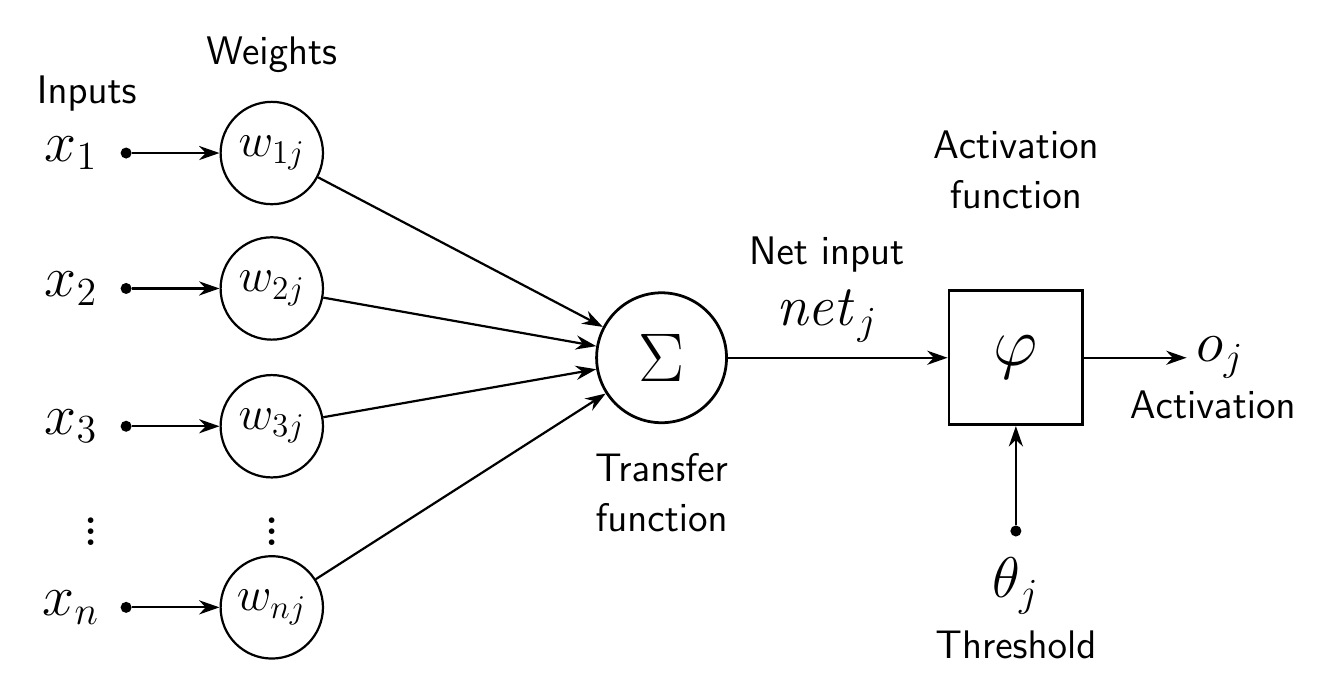
\begin{tikzpicture}[
    >={Stealth[length=2.6mm,width=1.8mm]},
    every node/.style={font=\sffamily\Large},
    weight/.style={circle, draw, line width=0.8pt, minimum size=1.3cm, inner sep=0pt},
    sumnode/.style={circle, draw, line width=1pt, minimum size=1.65cm, inner sep=0pt},
    actbox/.style={rectangle, draw, line width=1pt, minimum size=1.7cm, inner sep=0pt},
    dot/.style={circle, fill, inner sep=0pt, minimum size=4pt},
    line/.style={line width=0.8pt},
    sym/.style={font=\huge}
]

% ---------------- Inputs and weights ----------------
\foreach \i/\y in {1/6.45, 2/4.73, 3/2.98, n/0.68} {
    \node[sym] at (0.9,\y) {$x_{\i}$};
    \node[dot] (in\i) at (1.6,\y) {};
    \node[weight,font=\LARGE] (w\i) at (3.45,\y) {$w_{\i j}$};
    \draw[line,->] (in\i) -- (w\i);
}

% Vertical ellipses
\node[font=\Huge] at (1.15,1.75) {$\vdots$};
\node[font=\Huge] at (3.45,1.75) {$\vdots$};

% Column headings
\node at (1.1,7.2)  {Inputs};
\node at (3.45,7.7) {Weights};

% ---------------- Summation (transfer function) ----------------
\node[sumnode] (sum) at (8.4,3.85) {\Huge$\Sigma$};
\foreach \i in {1,2,3,n} {
    \draw[line,->] (w\i) -- (sum);
}
\node[align=center, below=0.25cm of sum] {Transfer\\function};

% ---------------- Activation function ----------------
\node[actbox] (phi) at (12.9,3.85) {\Huge$\varphi$};
\draw[line,->] (sum) -- (phi)
    node[sym, pos=0.45, above=2pt] {$\mathit{net}_j$}
    node[pos=0.45, above=0.95cm] {Net input};
\node[align=center, above=0.9cm of phi] {Activation\\function};

% ---------------- Output ----------------
\draw[line,->] (phi.east) -- ++(1.3,0) node[sym, right] {$o_j$};
\node at (15.4,3.25) {Activation};

% ---------------- Threshold ----------------
\node[dot] (th) at (12.9,1.65) {};
\draw[line,->] (th) -- (phi);
\node[sym] at (12.9,0.95) {$\theta_j$};
\node at (12.9,0.2)  {Threshold};

\end{tikzpicture}
\end{document}
